\documentclass[12pt]{beamer}  
\usepackage{xeCJK}  
\usepackage{mathdots}  
\usepackage{graphicx}  
\usepackage{float}  
\usepackage{multirow}  
%\usepackage{cite}  
\usepackage{amsfonts, amsmath, mathrsfs, amsbsy, amssymb, dsfont,setspace}
\usepackage[square, comma, sort&compress, numbers]{natbib} 
\usepackage{algorithm}  
\usepackage{algorithmic} 
\usepackage{float} 
\usepackage{latexsym} 
%\usetheme{Warsaw}  
\usetheme{CambridgeUS}
\begin{document} 
\title{低秩特性和联合稀疏的减弱墙体回波方法研究}  
\author{黄臣}  
\date{\today}  
\frame{\titlepage}  
\begin{frame}
  \frametitle{Low-Rank}
  如果$\bf X$是一个$m$行$n$列的数值矩阵,$\rm {rank(}\bf X\rm {)}$是$\bf X$的秩,
  假如$\rm {rank(}\bf X\rm {)}$远小于$m$和$n$,则我们称$\bf X$是低秩矩阵。
  秩可以度量相关性,当用少数几个线性无关的向量就可以表示整个矩阵时,说明矩阵
  具有低秩特性,在图像上,低秩特性表现为图像上的基底(字典)数目会很少。具体
  应用可以为拿来去除照片中的噪点,电影中的雨丝也可以通过低秩表达的方式来去除。

  而在穿墙雷达成像中,来自前墙的回波也被认为是具有低秩特性的矩阵,因此可以
  使用相关方法进行去除墙体回波。
\end{frame}
\begin{frame}
  \frametitle{Low-Rank}
  低秩矩阵逼近(LRMA)的方法被应用在很多地方,\citep{Ren2016Image}采用了一种
  加权核范数最小化的方法,用于先验盲图像去模糊。\citep{Tang2016Radar}则提
  出了一种迭代软阈值算法,用于使用减少的测量集来估计前墙回波的低秩矩阵和
  目标回波的稀疏矩阵。\citep{Bouzerdoum2017A}则是应用在了多极化信道的穿墙
  雷达成像上。
\end{frame}
\begin{frame}
  \frametitle{Soft thresholding algorithm}
  我们回波信号模型定为:
  \begin{equation} 
	\mathbf{Z}=\mathbf Z^{w}+\mathbf{Z}^{t}+\Upsilon.
  \end{equation}
  所以我们的目标为估计$\mathbf{Z}^w$和$\mathbf{Z}^{t}$,这里采用鲁棒主成分分析
  (RPCA),所以优化问题描述为:
  \begin{equation} 
	\mathop{\text{minimize}}\limits_{\mathbf{Z}^{w},\mathbf{Z}^{t}} \Vert \mathbf{Z}^{w}\Vert_{*}+\lambda\Vert \mathbf{Z}^{t}\Vert_{1}\ \; \mathbf{s.t}.\ \Vert \mathbf{Z}-(\mathbf{Z}^{w}+\mathbf{Z}^{t})\Vert_{2} < \epsilon 
  \end{equation}
  当$\mathbf{Z}$的全部数据被测量时,我们可以用凸优化的方法来解上式\citep{Chandrasekaran2009Rank}。 
\end{frame}
\begin{frame}
  \frametitle{Soft thresholding algorithm}
  在本例中,我们只测量了$K$个数据($K \ll N \times M$),记线性变换$\mathcal{A}$
  为$\mathbb{C}^{M\times\!N}\to\mathbb{C}^{K}$:
  \begin{equation*}
	\mathbf{y}=\mathcal{A}(\mathbf{Z})=\mathcal{A}(\mathbf{Z}^{w}+\mathbf{Z}^{t}+\Upsilon)
  \end{equation*}
  优化问题变为:
  \begin{equation}
	\mathop{\text{minimize}}\limits_{\mathbf{Z}^{w},\mathbf{Z}^{t}} \Vert \mathbf{Z}^{w}\Vert_{*}+\lambda\Vert \mathbf{Z}^{t}\Vert_{1}\ \mathbf{s.t}.\ \Vert \mathbf{y}-\mathcal{A}(\mathbf{Z}^{w}+\mathbf{Z}^{t})\Vert_{2} < \epsilon
  \end{equation}
  \citep{Waters2011SpaRCS}提出的SpaRSC贪婪算法,可用于解决该优化问题,但是需要
  有矩阵$\mathbf{Z}$的稀疏水平的先验知识。
\end{frame}
\begin{frame}
  \frametitle{Soft thresholding algorithm}
  我们引入稀疏字典$\mathbf{W}$来取代假设信号域的稀疏性,并将式(3)转化为拉格朗日
  正则化的形式:
  \begin{equation}
\mathop\text{minimize}\limits_{\mathbf{Z}^{w},\mathbf{Z}^{t}} \Vert \mathbf{y}-\mathcal{A}(\mathbf{Z}^{w}+\mathbf{Z}^{t})\Vert_{2}+\lambda_{w}(\Vert \mathbf{Z}^{w}\Vert_{*}+\lambda\Vert \mathbf{WZ}^{t}\Vert_{1})
  \end{equation}
  为解决上面的问题,我们引入迭代软阈值的算法,使$\mathbf{Z}^w$的奇异值和矩阵
  $\mathbf{WZ}^t$的项收缩到0,阈值算子为:
  \begin{equation*}
	\mathcal{T}_{\tau}(x)=\frac{x}{\vert x\vert }(\vert x\vert -\tau)_{+}
  \end{equation*}
\end{frame}
\begin{frame}
  \frametitle{Soft thresholding algorithm}
  \scriptsize
  \begin{algorithm}[H]  
	\caption{软阈值迭代}
	\label{alg:1}
	\begin{algorithmic}[1]
	  \STATE{初始化:$\tilde{\mathbf{Z}}_0=\mathcal{A}^Ty,\;\tilde{\mathbf{Z}}_0^w=\tilde{\mathbf{Z}_0},\; 
	  \tilde{\mathbf{Z}}_0^t=0,\;i=1$}
	  \STATE{Step 1:$\tilde{\mathbf{Z}}_{i}^{w}=\mathcal{S}_{\lambda_{w}}(\tilde{\mathbf{Z}}_{i-1}-\tilde{\mathbf{Z}}_{i-1}^{t})$}
	  \STATE{Step 2:$\tilde{\mathbf{Z}}_{i}^{t}=\mathbf{W}^{\dagger}(\mathcal{T}_{\lambda_{t}}\mathbf{W}(\tilde{\mathbf{Z}}_{i-1}-\tilde{\mathbf{Z}}_{i-1}^{w}))$}
	  \IF{$\frac{\Vert\tilde{\mathbf{Z}}_{i}^{w}+\tilde{\mathbf{Z}}_{i}^{t}-(\tilde{\mathbf{Z}}_{i-1}^{w}+\tilde{\mathbf{Z}}_{i-1}^{t})\Vert_{2}}{\Vert\tilde{\mathbf{Z}}_{i-1}^{w}+\tilde{\mathbf{Z}}_{i-1}^{t}\Vert_{2}} < \delta $}
	  \STATE{结束}
	  \ELSE
	  \STATE{$\tilde{\mathbf Z}_{i}=\tilde{\mathbf{Z}}_{i}^{w}+\tilde{\mathbf{Z}}_{i}^{t}-\mathcal{A}^{T}(\mathcal{A}(\tilde{\mathbf{Z}}_{i}^{w}+\tilde{\mathbf{Z}}_{i}^{t})-\mathbf{y})$}
	  \STATE{$i\leftarrow i+1 $}
	  \STATE{回到Step 1}
	  \ENDIF
	\end{algorithmic}
  \end{algorithm}
\end{frame}
\begin{frame}{Multipolarization Through-wall Radar}
  回波信号模型和前面相似:
  \begin{equation}
	\mathbf{Z}_l=\mathbf Z^{w}_l+\mathbf{Z}_l^{t}+\Upsilon_l
  \end{equation}
  其中$\mathbf{Z}_l$表示第$l$个极化信道的回波。优化问题转化为:
  \begin{equation}
	\mathop{\text{minimize}}\limits_{\mathbf{Z}^{w},\mathbf{S}} \Vert \mathbf{Z}^{w}\Vert_{*}+\lambda\Vert \mathbf{S}^T\Vert_{2,1}\ \mathbf{s.t}.\ \Big\Vert \mathbf{Y}-\big[\mathcal{A}(\mathbf{Z}^{w})+\Phi\Psi\mathbf{S}\big]\Big\Vert_{F}^2 < \epsilon
  \end{equation}
  其中$\mathcal A(\mathbf{Z}^w) = [\Phi\mathbf{vec}(\mathbf{Z}_1^w),\dots,\Phi\mathbf{vec}(\mathbf{Z}_L^w)] $,$\Phi$为稀疏字典,$\Psi\mathbf S = \mathbf Z^t$。
\end{frame}
\begin{frame}{Multipolarization Through-wall Radar}
  转化(6)为拉格朗日形式:
  \begin{equation}
	\frac{1}{2}\Big\Vert \mathbf{Y}-\big[\mathcal{A}(\mathbf{Z}^{w})+\Phi\Psi\mathbf{S}\big]\Big\Vert_{F}^2 +\gamma\big(\Vert \mathbf{Z}^{w}\Vert_{*}+\lambda\Vert \mathbf{S}^T\Vert_{2,1}\big) 
  \end{equation}
  对于形如$\mathop{\text{minimize}}\limits_{\mathbf x}f(\mathbf x)=g(\mathbf x)+\lambda h(\mathbf x)$的优化问题,其中$g(\mathbf x)$为凸函数且光滑可微,$h(\mathbf x)$凸但不严格光滑,可采用迭代估计每一次的$\mathbf x_i$的值来求解:
  \begin{equation*}
	\mathbf x_{i+1} = \mathop{\text{minimize}}\limits_{\mathbf x}\frac{1}{2}\Vert \mathbf u_i -\mathbf x \Vert _2^2+\lambda \alpha h(\mathbf x) 
  \end{equation*}
  其中$\mathbf u_i = \mathbf x_i -\alpha\nabla g(\mathbf x_i)$,当$\alpha\in\big(0,\frac{1}{C}\big]$将收敛。
\end{frame}
\begin{frame}{Multipolarization Through-wall Radar}
  优化问题可分解为:
  \begin{eqnarray}
  \mathbf{Z}_{i+1}^w&=&\mathop{\text{minimize}}\limits_{\mathbf{Z}^{w}}\frac{1}{2}\Big\Vert \mathbf{Z}_i-\mathbf{Z}^{w}-\mathcal{A}^*(\Phi\Psi\mathbf{S}_i)\Big\Vert_{F}^2 +\alpha\gamma\Vert\mathbf{Z}^{w}\Vert_{*}\\ 
	\mathbf{S}_{i+1}^w&=&\mathop{\text{minimize}}\limits_{\mathbf{s}}\frac{1}{2}\Big\Vert \mathbf{Z}_{i}-\mathbf{Z}^{w}_{i+1}-\mathcal{A}^*(\Phi\Psi\mathbf{S})\Big\Vert_{F}^2 +\alpha\gamma\lambda\Vert\mathbf{Z}^{w}\Vert_{*} 
  \end{eqnarray}
收敛条件为$\alpha\in\big(0,1/\Vert \Phi \Vert_2^2\big]$,其中(9)式可以进一步写为:
\begin{equation}
  \mathbf{S}_{i+1} = \mathop{\text{minimize}}\limits_{\mathbf{s}} \frac{1}{2}\Vert \mathbf{X}-\mathbf{S}\Vert_F^2+\beta\alpha\gamma\lambda\Vert\mathbf{S}^T\Vert_{2,1}
\end{equation}
其中:
\begin{equation*}
  \mathbf{X}=\mathbf S_i -\beta \Psi^H( \Phi \Psi\mathbf S_i-\mathcal A(\mathbf Z_i-\mathbf Z_{i+1}^w))
\end{equation*}
\end{frame}
\begin{frame}{Multipolarization Through-wall Radar}
  和算法\ref{alg:1}类似,多极化信道下的迭代算法为:
  \begin{algorithm}[H]  
 % \algsetup{linenosize=\footnotesize} 
  \footnotesize
	\caption{多极化信道下的软阈值迭代}
	\label{alg:2}
	\begin{algorithmic}[1]
	  \STATE{初始化:$\mathbf{Z}_0^w\gets\mathcal{A}^*(\mathbf Y),\;\mathbf{S}_0 \gets 0,\;i\gets 0$}
	  \STATE{Step 1:$\mathbf{Z}_i\gets \mathbf{Z}_i^w+\mathcal{A}^*(\Phi\Psi\mathbf{S}_i)-\alpha\mathcal{A}^*(\mathcal{A}(\mathbf{Z}_i^w)+\Phi\Psi\mathbf{S}_i-\mathbf{Y})$}
	  \STATE{Step 2:$\mathbf{Z}_{i+1}^w\gets\mathcal{S}_{\alpha\gamma}(\mathbf{Z}_i-\mathcal{A}^*(\Phi\Psi\mathbf{S}_i))$}
	  \STATE{Step 3:$\mathbf{X}\gets\mathbf S_i -\beta \Psi^H( \Phi \Psi\mathbf S_i-\mathcal A(\mathbf Z_i-\mathbf Z_{i+1}^w))$}
	  \STATE{Step 4:$\mathbf{S}_{i+1}\gets\mathcal{R}_{\beta\alpha\gamma\lambda}(\mathbf{X})$}
	  \IF{$\frac{\vert f(\mathbf{Z}_{i+1}^w,\mathbf{S}_{i+1})-f(\mathbf{Z}_{i}^w,\mathbf{S}_i)\vert }{\vert f(\mathbf{Z}_i^w,\mathbf{S}_i)\vert} < \delta $}
	  \STATE{结束}
	  \ELSE
	  \STATE{$i\leftarrow i+1 $}
	  \STATE{回到Step 1}
	  \ENDIF
	\end{algorithmic}
  \end{algorithm}
\end{frame}
\begin{frame}[allowframebreaks]{References}
 % \footnotesize
  \scriptsize
  \bibliographystyle{ieeetr} 
  \bibliography{ct.bib} 
\end{frame}
\end{document}
\begin{frame}
  \frametitle{Compressive Sensing Based Scene Reconstruction}
\end{frame}
\begin{frame}
  \frametitle{Compressive Sensing Based Scene Reconstruction}
\end{frame}
\begin{frame}
  \frametitle{Compressive Sensing Based Scene Reconstruction}
\end{frame}
\begin{frame}
  \frametitle{Compressive Sensing Based Scene Reconstruction}
\end{frame}
\*begin{figure}[H]
\centering
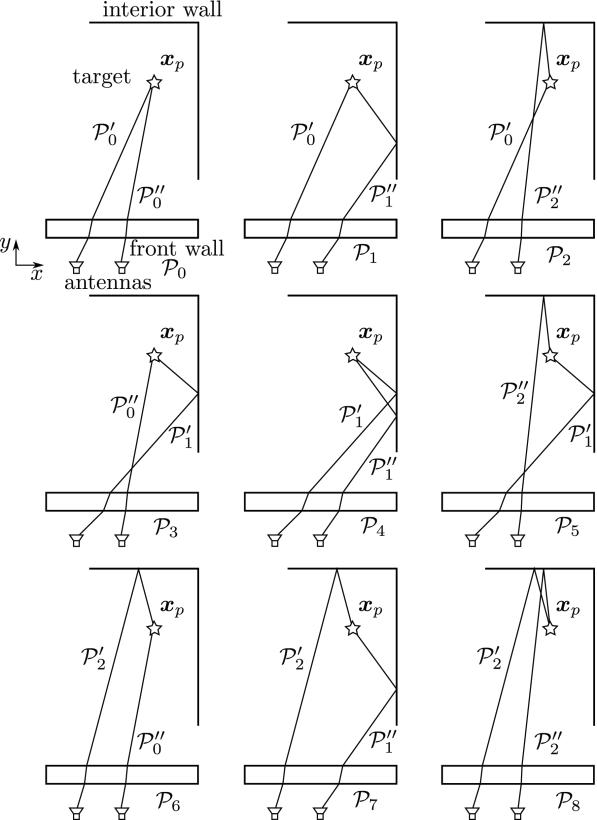
\includegraphics[width=0.5\mathbfwidth]{fig2}
\caption{CSI处理流程图}
\end{figure}
